\section{Results}

\subsection{Reproducing the published baselines (E1)}

With the paper's split, feature sets (including the time step) and stated
hyper-parameters, our Random Forest reaches an illicit F1 of \RepRFAF{}
($\pm$\RepRFAFSd{} over five seeds) on all features, against 0.788 published
(Fig.~\ref{fig:repro}). On local features we obtain \RepRFLF{}, above the
published 0.694. The MLP on local features matches (\RepMLPLF{} vs 0.649); on all
features it is lower (\RepMLPAF{} vs 0.653), a gap we attribute to unreported
training details (batch size, initialisation, input scaling). Logistic
Regression stays below the paper (\RepLRAF{} vs 0.481) even with the 2019
scikit-learn defaults. The ranking of models, which is what the paper's
conclusions rest on, is reproduced: Random Forest $>$ MLP $>$ Logistic Regression.

\begin{figure}[t]
  \centering
  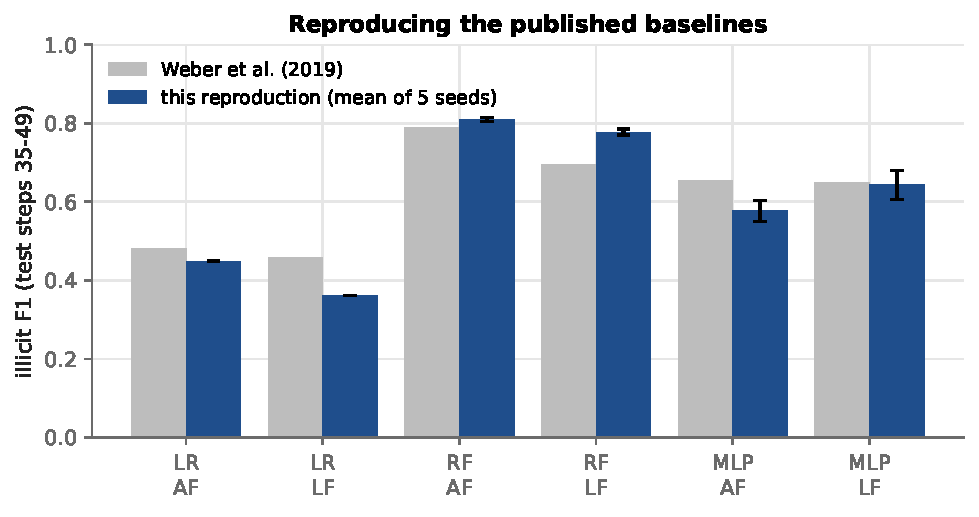
\includegraphics[width=\columnwidth]{../reports/figures/e01_reproduction.pdf}
  \caption{Illicit F1 of the published baselines~\cite{weber2019} and of our
  reproduction (mean and standard deviation over five seeds).}
  \label{fig:repro}
\end{figure}

\subsection{Model comparison under a fair protocol (E2)}

Table~\ref{tab:main} gives the main comparison on all 165 features without
the time step, with tuned hyper-parameters and validation-chosen thresholds.
Random Forest (F1 \MainRFFone{}) and XGBoost (\MainXGBFone{}) are
\emph{statistically tied}: the paired bootstrap gives $p\PairedXGBRFFoneP{}$ for
F1 and $p\PairedXGBRFPRAUCP{}$ for PR-AUC. Both are clearly better than the MLP
(\MainMLPFone{}) and Logistic Regression (\MainLRFone{}), with $p<0.001$.

\begin{table}[t]
  \centering
  \caption{Test results (steps 35--49), mean of five seeds. CIs are 95\%
  block-bootstrap intervals over time steps. Budget: share of illicit
  transactions found by reviewing the top 100 per step.}
  \label{tab:main}
  \setlength{\tabcolsep}{3pt}
  \footnotesize
  \begin{tabular}{lcccc}
    \toprule
    Model & F1 [95\% CI] & PR-AUC [95\% CI] & Prec. / Rec. & Budget \\
    \midrule
    RF      & \MainRFFone{}  {\scriptsize\MainRFFoneCI{}}  & \MainRFPRAUC{}  {\scriptsize\MainRFPRAUCCI{}}  & \MainRFPrecision{} / \MainRFRecall{}   & \MainRFBudget{} \\
    XGBoost & \MainXGBFone{} {\scriptsize\MainXGBFoneCI{}} & \MainXGBPRAUC{} {\scriptsize\MainXGBPRAUCCI{}} & \MainXGBPrecision{} / \MainXGBRecall{} & \MainXGBBudget{} \\
    MLP     & \MainMLPFone{} {\scriptsize\MainMLPFoneCI{}} & \MainMLPPRAUC{} {\scriptsize\MainMLPPRAUCCI{}} & \MainMLPPrecision{} / \MainMLPRecall{} & \MainMLPBudget{} \\
    LR      & \MainLRFone{}  {\scriptsize\MainLRFoneCI{}}  & \MainLRPRAUC{}  {\scriptsize\MainLRPRAUCCI{}}  & \MainLRPrecision{} / \MainLRRecall{}   & \MainLRBudget{} \\
    \bottomrule
  \end{tabular}
\end{table}

The confidence intervals are the most sobering part of the table. The interval
for the best F1 spans more than 0.25. The test period contains 15 time steps,
not 16,670 independent transactions, and the steps differ wildly in difficulty
(Section~\ref{sec:drift}). Differences of a few hundredths between models, the
scale at which much of the literature on this dataset ranks methods, are well
inside this uncertainty unless tested with a paired design as we do here.
